% CVPR 2027 submission (review format). Built on the official author kit.
% Tables are generated from results_pilot/ by scripts/make_tex.py (tab_*.tex);
% every number quoted in the text is checked by scripts/verify_paper_numbers.py.
\documentclass[10pt,twocolumn,letterpaper]{article}
\usepackage[review]{cvpr}
\usepackage{graphicx,booktabs,amsmath,amssymb,multirow}
\usepackage{microtype}
%% This file contains a number of tweaks that are typically applied to the main document.
%% They are not enabled by default, but can be enabled by uncommenting the relevant lines.


%%
%% Official support for 2-column teaser figure
%%
\usepackage{cuted} %< for strip environment

%%
%% For auto-referencing of figures (see fig/teaser.tex and \label{} therein) 
%%
\usepackage{currfile} %< for \currfilebase macro

%%
%% caption and (global) spacing overrides
%%
\usepackage{caption} %< for "\captionof" commands (teaser)
% \setlength{\abovecaptionskip}{.5em} % space above caption
% \setlength{\belowcaptionskip}{1em} % space below caption

%%
%% Inline annotations; for predefined colors, refer to "dvipsnames" in the xcolor package:
%% https://tinyurl.com/overleaf-colors
%%
\newcommand{\red}[1]{{\color{red}#1}}
\newcommand{\todo}[1]{{\color{red}#1}}
\newcommand{\TODO}[1]{\textbf{\color{red}[TODO: #1]}}
%%
%% Disable for camera ready / submission by uncommenting these lines:
%%
% \renewcommand{\TODO}[1]{}
% \renewcommand{\todo}[1]{#1}

%%
%% Work harder in optimizing text layout. Typically shrinks text by 1/6 of page, enable
%% it at the very end of the writing process, when you are just above the page limit.
%%
% \usepackage{microtype}

%%
%% Fine-tune paragraph spacing.
%%
% \renewcommand{\paragraph}[1]{\vspace{.5em}\noindent\textbf{#1.}}

%%
%% Globally adjusts space between figure and caption.
%%
% \setlength{\abovecaptionskip}{.5em}

%%
%% Allows "the use of \paper to refer to the project name"
%% with automatic management of space at the end of the word.
%%
% \usepackage{xspace}
% \newcommand{\paper}{ProjectName\xspace}

%%
%% Commonly used math definitions.
%%
% \DeclareMathOperator*{\argmin}{arg\,min}
% \DeclareMathOperator*{\argmax}{arg\,max}

%%
%% Tighten underline.
%%
% \usepackage{soul}
% \setuldepth{foobar}

%%
%% Reconfigure paragraph (tweaks spacing)
%%

\definecolor{cvprblue}{rgb}{0.21,0.49,0.74}
\usepackage[pagebackref,breaklinks,colorlinks,allcolors=cvprblue]{hyperref}
\def\confName{CVPR}
\def\confYear{2027}
\newcommand{\Areal}{A_{\text{real}}}
\newcommand{\Atext}{A_{\text{text}}}
\newcommand{\FDD}{\text{FD}_{\text{DINO}}}

\title{What Makes Synthetic Training Data Work?\\
A Pilot Interventional Study on Fine-Grained Classification}
\author{Anonymous CVPR submission}

\begin{document}
\twocolumn[{%
\renewcommand\twocolumn[1][]{#1}%
\maketitle
\centering
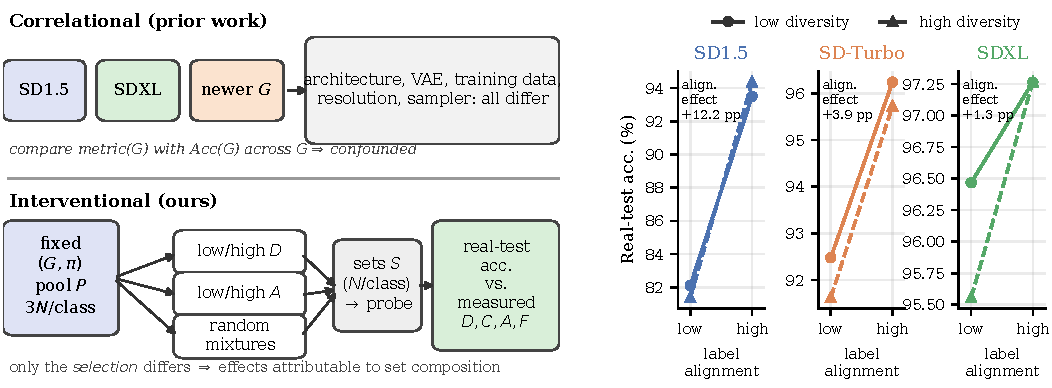
\includegraphics[width=\linewidth]{figs/fig1.pdf}
\captionof{figure}{\textbf{Left:} cross-generator comparisons change everything at once; we instead fix the generator $G$ and prompt regime $\pi$ and vary only \emph{which} images form the training set. \textbf{Right:} a $2{\times}2$ intervention on 20 CUB-200 classes. Raising label alignment lifts real-test accuracy by $+12.2$, $+3.9$ and $+1.3$ points for SD1.5, SD-Turbo and SDXL; raising diversity does not help ($-0.7$ to $+0.1$). The fixable deficit of synthetic data is \emph{correctness}, and it shrinks as generators improve. Note the per-panel $y$-scales.}
\label{fig:hook}
\vspace{1em}
}]

\begin{abstract}
Newer text-to-image generators produce prettier images that can train \emph{worse} classifiers, a regression recently attributed to a collapse of diversity and label alignment~\cite{adamkiewicz2026pretty}. That diagnosis rests on comparing generators, which differ in architecture, autoencoder, training data and sampler all at once. We ask which property of a synthetic training set actually drives real-test accuracy, and we answer by \emph{intervention}: with generator, prompt and image pool held fixed, we build equal-sized training sets that differ in one measured property (intrinsic diversity, coverage, label alignment or per-sample fidelity) using a $2{\times}2$ factorial and a randomized subset design with Shapley attribution. In a compute-limited study on 20 fine-grained CUB-200-2011 classes with three open generators and a frozen DINOv2 probe, we find: (i) the generational regression does \emph{not} replicate; SDXL is the best teacher (96.2\% vs.\ 90.9\% for SD1.5, $p{<}0.001$). (ii) Within a pool, label alignment is the lever ($+12.2$, $+3.9$, $+1.3$ points), its effect shrinking with generator quality, while increasing diversity never helps. (iii) The remaining gap is concentrated in a few classes, two of which account for 58--82\% of it, and a CLIP text scorer can be confidently wrong about them. (iv) A training-free recipe, DAS (oversample, filter by alignment, select for coverage), improves on random selection in 6/6 settings by 1.2--3.4 points without real images, yet a plain alignment filter is about as good, and five real images per class still beat every synthetic set. We report each result with its uncertainty and list what the pilot scale cannot support.
\end{abstract}

%-------------------------------------------------------------------------
\section{Introduction}
Text-to-image (T2I) models are an appealing source of training data: cheap to query, free of collection cost, and in principle able to depict any class in any condition~\cite{azizi2023synthetic,he2023synthetic,rombach2022high,sariyildiz2023fake}. One would expect better generators to yield better data. Adamkiewicz et al.~\cite{adamkiewicz2026pretty} showed the opposite: across thirteen open generators released between 2022 and 2025, classifiers trained only on synthetic ImageNet images get steadily worse on real test images with newer models, even as visual quality and prompt following improve. Their analysis traces the regression to a collapse toward a narrow, aesthetic-centric distribution that undermines diversity and label--image alignment.

This observation leaves three questions open for anyone who wants to \emph{use} synthetic data. \emph{First}, the evidence is correlational. Two generators differ in architecture, autoencoder, training corpus, resolution and guidance behaviour simultaneously, so an association between, say, coverage and accuracy across generators cannot isolate coverage. \emph{Second}, it concerns generic ImageNet classes that generators have seen countless times. In fine-grained domains a generator may render a beautiful, varied image of the \emph{wrong species}, and label alignment rather than diversity may bind. \emph{Third}, it offers no remedy that does not presuppose real data.

We change the method rather than the scale: we \emph{intervene on the training set} instead of comparing generators (Fig.~\ref{fig:hook}, left). For a fixed generator and prompt regime we draw a pool of $3\times$ more images than needed and build many training sets of identical size from it, differing systematically in one measured property. Because generator, prompt, autoencoder and resolution are constant, accuracy differences are attributable to the composition of the set. This forces distinctions that correlational studies blur: intrinsic diversity (Vendi~\cite{friedman2023vendi}) is not coverage of the real distribution~\cite{kynkaanniemi2019improved,naeem2020reliable}; label alignment is not prompt following; per-sample fidelity is not FID~\cite{heusel2017gans,kynkaanniemi2023role}.

\paragraph{Findings.} On 20 CUB-200-2011~\cite{wah2011cub} classes with SD1.5, SD-Turbo and SDXL:
\begin{itemize}\setlength\itemsep{0pt}\setlength\topsep{2pt}
\item \textbf{No generational regression here.} SDXL trains the best classifier, and of the standard generator metrics only $\FDD$ ranks the three generators as their data does; precision ranks the worst teacher first (Sec.~\ref{sec:cross}).
\item \textbf{Correct before diverse.} Holding the pool fixed, raising label alignment lifts accuracy by up to 12.2 points; raising diversity does not help, and alignment-filtered sets are \emph{less} diverse yet better (Fig.~\ref{fig:hook}, Sec.~\ref{sec:factorial}).
\item \textbf{The gap lives in a few classes} that the generator does not know, and CLIP-based familiarity can be confidently wrong about them (Sec.~\ref{sec:h3}).
\item \textbf{DAS} (Diversity-matched, Alignment-filtered Sampling), a training-free selection rule, beats random selection in every setting and beats using all $3\times$ images in 5/6, but most of its gain comes from the filter (Sec.~\ref{sec:das-res}).
\end{itemize}

\paragraph{Contributions.} (1) An interventional protocol that decomposes the synthetic-to-real gap into diversity, coverage, alignment and fidelity with the generator held fixed, including manipulation checks and an autoencoder-reconstruction control. (2) Evidence from a fine-grained domain that the dominant, fixable factor is label alignment and that its weight shrinks with generator quality. (3) DAS and a compute-matched comparison against its natural ablations. (4) Methodological safeguards we found necessary: leak-free alignment scoring, disjoint selection (CLIP) and measurement (DINOv2) embeddings, a real-data-free validation protocol, and test-set uncertainty on every comparison. We wrote down four hypotheses before running the interventions (Sec.~\ref{sec:hyp}) and report negative outcomes as findings.

\paragraph{Scope.} The full design (four generators including SD3.5 and FLUX.1-dev, two datasets, three generation seeds) needs $\approx$600 A100-hours. This paper reports a pilot run: generation on free Kaggle T4 GPUs (15\,GB), all analysis on a laptop; every claim is scoped to it and Sec.~\ref{sec:limits} lists what was not run.

%-------------------------------------------------------------------------
\section{Related work}
\paragraph{Training on generated images.} Diffusion images can train or pretrain useful classifiers: ImageNet clones from Stable Diffusion~\cite{sariyildiz2023fake}, synthetic data for zero- and few-shot recognition~\cite{he2023synthetic}, fine-tuned Imagen data~\cite{azizi2023synthetic}, and synthetic contrastive pretraining~\cite{tian2023stablerep,tian2024learning}. Fan et al.~\cite{fan2024scaling} chart scaling laws and their limits; Geng et al.~\cite{geng2024unmet} show retrieving real images from a generator's training set beats generating; Singh et al.~\cite{singh2024synthetic} benchmark robustness. Adamkiewicz et al.~\cite{adamkiewicz2026pretty} extend the comparison to thirteen generators and find the regression we revisit. Their study is correlational across generators on generic classes; ours intervenes within generators on fine-grained classes and proposes a remedy.

\paragraph{Diversity, prompts and conditioning.} Synthetic data is often said to lack diversity, and many methods act on the prompt or the generator: diversified prompts~\cite{shipard2023diversity}, captions as prompts~\cite{lei2023image}, editing real images toward new domains~\cite{dunlap2023diversify,trabucco2024effective}, structure-preserving generation for fine-grained classes~\cite{michaeli2024advancing}, few-shot generator fine-tuning~\cite{kim2024datadream}, and distribution matching~\cite{yuan2024realfake}. DAS is complementary: it leaves the generator untouched and only decides which samples to keep, so it can be stacked on any of these.

\paragraph{Selection, label noise and generative metrics.} Greedy $k$-center coresets~\cite{gonzalez1985clustering,sener2018active}, difficulty-based pruning~\cite{sorscher2022beyond} and agreement-based label-noise filtering~\cite{northcutt2021confident} are established for real data; a misaligned synthetic image is label noise whose rate depends on how well the generator knows the class. FID~\cite{heusel2017gans} and KID~\cite{binkowski2018demystifying} mix fidelity and diversity and inherit ImageNet bias from Inception features~\cite{kynkaanniemi2023role}; precision/recall~\cite{kynkaanniemi2019improved} and density/coverage~\cite{naeem2020reliable} separate them, DINOv2 features~\cite{oquab2024dinov2} are preferable to Inception~\cite{stein2023exposing}, and Vendi~\cite{friedman2023vendi} measures diversity without a reference. We use these metrics as candidate \emph{explanatory variables} and test which ones matter under intervention.

%-------------------------------------------------------------------------
\section{Study design}
\paragraph{Notation.} A task has $K$ classes, a real training set $D_r$ and a real test set $D_\text{te}$ used only for final evaluation. Generator $G$ with prompt regime $\pi$ yields a pool $P_{G,\pi}$ of $mN$ images per class ($m{=}3$). A training set $S\subset P$ has exactly $N$ images per class, with $N$ the per-class size of $D_r$, so synthetic and real sets are equal in size. Before anything else we carve an \emph{alignment split} $A\subset D_r$ of $k{=}5$ images per class and remove it from $D_r$; it is used only to score alignment and to train the matched real 5-shot baseline, so no method that sees $A$ is compared to a classifier denied it.

\subsection{Data, generators and prompts}
\paragraph{Data.} CUB-200-2011~\cite{wah2011cub} is fine-grained: species differ in local plumage cues and are rare in web captions. We use 20 classes at evenly spaced indices (no hand-picking), with $N{=}24$ real training images per class after carving $A$ and 585 test images (one image $=0.17$ points).

\paragraph{Generators.} SD1.5~\cite{rombach2022high}, SD-Turbo, an adversarially distilled model~\cite{sauer2024adversarial}, and SDXL~\cite{podell2024sdxl}. SD3.5~\cite{esser2024scaling,stability2024sd35} and FLUX.1-dev~\cite{bfl2024flux} did not fit the 15\,GB GPUs available. SD1.5 and SDXL use 25 steps and classifier-free guidance~\cite{ho2022classifier} of 2.0, the low-guidance setting known to favour diversity~\cite{adamkiewicz2026pretty,rombach2022high}; SD-Turbo uses 4 steps without guidance. SD1.5 and SD-Turbo run at $512^2$, SDXL at $768^2$ (below its native $1024^2$, for memory). Steps, guidance and resolution are thus confounded with the generator, which is precisely why our main analyses are within-generator. All images are resized to $224^2$.

\paragraph{Prompts.} \textbf{P1}: ``a photo of a \{class\}, a type of bird''. \textbf{P2}: LLM-written templates varying pose, background, lighting, season and viewpoint, always containing the class name, written once per domain without access to real images. Each pool holds 72 images per class (1,440 per pool, six pools); every training set has 480 images.

\subsection{Measured properties}\label{sec:measures}
All set-level metrics are computed per class at equal $N$ and averaged, because several depend on sample size. Measurements use DINOv2 ViT-B/14~\cite{oquab2024dinov2}; \emph{selection} uses OpenCLIP ViT-L/14~\cite{radford2021learning}, so no selection rule can win by optimizing the space it is scored in.

\paragraph{Diversity $D$ (reference-free).} The Vendi score~\cite{friedman2023vendi}, $\exp$ of the entropy of the eigenvalues of $\tfrac1N\mathbf K$ for the cosine kernel $\mathbf K$: the effective number of distinct samples, with no reference to real data.

\paragraph{Coverage $C$ (reference-based).} The fraction of real images whose 5-NN ball contains a synthetic image~\cite{naeem2020reliable}, and improved recall~\cite{kynkaanniemi2019improved} ($k{=}3$). A set can raise Vendi by spreading into regions real data never occupies without raising coverage.

\paragraph{Label alignment $A$.} Two independent scorers $a(x,y)\in[0,1]$ for image $x$ prompted with class $y$, both in CLIP space. $\Areal$: softmax probability of $y$ under a nearest-class-mean classifier on the alignment split (temperature calibrated on that split; ties favour the softest temperature, so scores are flat and are used only through ranks and quantiles). $\Atext$: CLIP zero-shot probability over the $K$ class names, using no real image.

\paragraph{Fidelity $F$ (per sample).} Improved precision~\cite{kynkaanniemi2019improved} and density~\cite{naeem2020reliable}. We also report $\FDD$~\cite{stein2023exposing}, treated as a proxy to be tested, since it mixes fidelity and diversity.

\subsection{Learner and controls}
\paragraph{Frozen DINOv2 linear probe.} Multinomial logistic regression on $\ell_2$-normalized DINOv2 [CLS] features~\cite{kornblith2019better}, with weight decay chosen on a held-out \emph{synthetic} split (selecting on real validation data would leak real information). The probe measures images as supervision for a head on a real-pretrained backbone, not as pretraining data, and is cheap enough for the hundreds of trainings the designs require.

\paragraph{Controls.} Real-only training at 5, 10 and all images per class. An \emph{autoencoder ceiling}: real training images passed through a generator's VAE (encode--decode, no diffusion) bound how much of the gap latent-space artifacts alone can explain~\cite{adamkiewicz2026pretty}. \emph{Uncertainty:} all models share one 585-image test set; we give Wilson 95\% intervals for accuracies and mark differences significant under an unpaired two-proportion test, which is conservative relative to a paired test.

\subsection{Hypotheses}\label{sec:hyp}
These four hypotheses were written in our study plan \emph{before} the interventional experiments were run.
\begin{description}\setlength\itemsep{0pt}\setlength\topsep{2pt}
\item[H1] Within a fixed pool, coverage and alignment explain more variance in accuracy than per-sample fidelity, and Vendi explains less than coverage.
\item[H2] Across generators, newer models score higher on fidelity and lower on coverage under P1, so FID and precision mis-rank generators as data sources.
\item[H3] The gap is larger for classes the generator knows poorly, measured by class familiarity (mean $\Atext$ under P1).
\item[H4] Alignment filtering followed by coverage selection closes a meaningful share of the gap, beyond training on the whole oversampled pool.
\end{description}

%-------------------------------------------------------------------------
\section{From correlation to intervention}
Fixing $(G,\pi)$ fixes the autoencoder, resolution, sampler and training corpus. We vary only which $N$ images per class are kept, so the manipulated variable is the composition of the training set; its effect is identified up to unmeasured properties that travel with our selection rules (Sec.~\ref{sec:limits}).

\paragraph{Diversity arm.} Keep images above the pool's 40th percentile of $\Areal$, then pick $N$ per class by \emph{clustered} selection (the $N$ nearest neighbours of a random image; low diversity) or greedy farthest-point $k$-center~\cite{gonzalez1985clustering} (high diversity). Since $k$-center favours outliers, we measure precision in every cell.

\paragraph{Alignment arm.} Draw randomly from the bottom or top tercile of $\Areal$. High-alignment images tend to be prototypical and less diverse, so within each tercile we draw 200 candidate subsets and keep the one whose Vendi is closest to the pool median.

\paragraph{$2{\times}2$ factorial.} Crossing the two arms gives four sets per $(G,\pi)$, each trained with three selection and three training seeds. An interaction is plausible a priori: diversity may only help when labels are correct, since spreading misaligned images adds varied label noise.

\paragraph{Randomized subsets and Shapley attribution.} To attribute variance across all four factors, we draw $R{=}150$ subsets per pool by mixing random, $k$-center, clustered and quantile-restricted draws in random proportions, and fit
\begin{equation}
\text{Acc}(S)=\beta_D\tilde D+\beta_C\tilde C+\beta_A\tilde A+\beta_F\tilde F+\gamma_{G,\pi}+\varepsilon,\label{eq:reg}
\end{equation}
with standardized regressors and a fixed effect $\gamma$ per pool, so variance is explained only \emph{within} pools. We report each factor's Shapley (LMG) share of $R^2$~\cite{gromping2006relative,lipovetsky2001analysis}, its average marginal contribution over all regressor orderings, which stays interpretable under correlated regressors.

%-------------------------------------------------------------------------
\section{DAS: Diversity-matched, Alignment-filtered Sampling}
DAS turns the decomposition into a recipe that needs no gradient step on the generator. For each class $y$: \textbf{(1) Oversample} $mN$ images ($m{=}3$) under P2. \textbf{(2) Filter} images with $a(x,y)<\tau$, $\tau$ the pool's 40th percentile (chosen on synthetic validation data); if fewer than $N$ survive, keep the top-$N$ by alignment. \textbf{(3) Select} $N$ survivors by greedy $k$-center in CLIP space~\cite{gonzalez1985clustering,sener2018active}, seeded with the most aligned survivor. DAS-real uses $\Areal$ (5 real images per class); DAS-text uses $\Atext$ and no real image anywhere. Selection costs $O(mN^2)$ distances per class, negligible next to generation.

DAS must beat \emph{Random-$N$}; \emph{All-$mN$}, the full pool, with $3\times$ the images at the same generation cost, which separates the value of selecting from the value of having more; \emph{Filter-only} and \emph{$k$-center-only}; and \emph{Real 5-shot}, the same real images DAS-real sees, used directly. We summarize each method by the fraction of the gap it closes,
\begin{equation}
\Delta=\frac{\text{Acc}(\text{method})-\text{Acc}(\text{Random-}N)}{\text{Acc}(\text{Real-}N)-\text{Acc}(\text{Random-}N)}.\label{eq:delta}
\end{equation}

%-------------------------------------------------------------------------
\section{Results}
\subsection{Cross-generator picture (H2)}\label{sec:cross}
\paragraph{The generational regression does not replicate at this scale.} Under P1, SDXL reaches 96.2\%, against 90.9\% for SD1.5 and 91.5\% for SD-Turbo (Tab.~\ref{tab:main}); SDXL's lead is significant ($p{<}0.001$ against each), the other difference is not ($p{=}0.76$). Kendall's $\tau$ between release order and accuracy is $+0.33$ under both prompt regimes, so there is no monotone decline. With three generators, none of them the 2024--25 models at the centre of~\cite{adamkiewicz2026pretty}, we read this as evidence that the regression is not universal on fine-grained data, not as evidence that it is absent.

\begin{table*}[t]
\centering\small
\setlength{\tabcolsep}{2.5pt}
\begin{tabular}{@{}llcrrrrrr@{}}
\toprule
Training data (480 images) & Prompt & Real-test acc.\ (\%) $\uparrow$ & FD$_\text{DINO}$ $\downarrow$ & Precision $\uparrow$ & Density $\uparrow$ & Coverage $\uparrow$ & Vendi $\uparrow$ & $A_\text{text}$ $\uparrow$ \\
\midrule
Real, 5/class & -- & 97.9 [96.4,98.8] & -- & -- & -- & -- & -- & -- \\
Real, 10/class & -- & 97.6 [96.0,98.6] & -- & -- & -- & -- & -- & -- \\
Real, all ($\approx$24/class) & -- & 98.6 [97.3,99.3] & -- & -- & -- & -- & -- & -- \\
\midrule
SD1.5 & P1 & 90.9 [88.3,93.0] & 0.93 & 0.62 & 0.04 & \textbf{0.70} & 11.2 & 0.73 \\
 & P2 & 90.6 [88.0,92.7] & 1.10 & \textbf{0.79} & 0.03 & 0.68 & \textbf{14.3} & 0.62 \\
\midrule
SD-Turbo & P1 & 91.5 [88.9,93.5] & 0.81 & 0.03 & 0.10 & 0.03 & 4.6 & 0.89 \\
 & P2 & 93.8 [91.6,95.5] & 0.93 & 0.18 & 0.05 & 0.25 & 8.5 & 0.77 \\
\midrule
SDXL ($768^2$) & P1 & \textbf{96.2} [94.4,97.5] & \textbf{0.74} & 0.27 & \textbf{0.11} & 0.36 & 6.5 & \textbf{0.92} \\
 & P2 & 95.9 [94.0,97.2] & 0.83 & 0.47 & 0.07 & 0.58 & 9.0 & 0.86 \\
\midrule
VAE recon.\ (SD1.5) & -- & 98.3 [96.9,99.1] & 0.11 & 0.98 & 0.88 & 1.00 & 5.2 & -- \\
VAE recon.\ (SD-Turbo) & -- & 98.5 [97.1,99.2] & 0.11 & 0.98 & 0.91 & 1.00 & 5.2 & -- \\
\bottomrule
\end{tabular}
\caption{\textbf{Cross-generator picture} (20 CUB classes, frozen DINOv2 probe, random selection, one generation seed). Brackets: Wilson 95\% intervals over the 585 test images. Bold: best synthetic value per column. Generator metrics are per-class averages in DINOv2 space. Precision ranks SD1.5, the worst teacher, first; only FD$_\text{DINO}$ orders the three generators as their accuracy does. VAE recon.: real training images re-rendered through the generator's autoencoder (not run for SDXL).}
\label{tab:main}
\end{table*}


\begin{figure*}[t]
\centering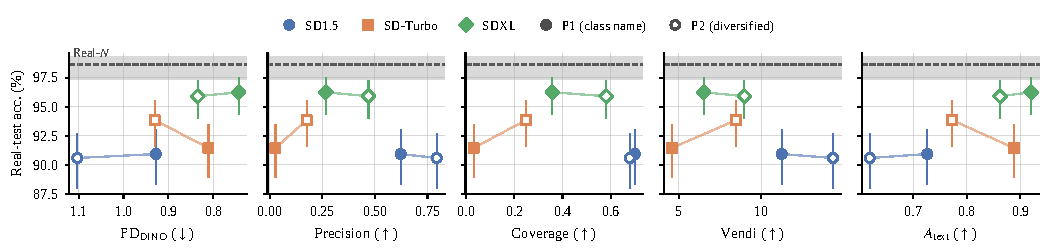
\includegraphics[width=\textwidth]{figs/fig2.pdf}
\caption{\textbf{Which generator metric predicts training utility?} Real-test accuracy against five generator-level metrics for three generators under P1 (filled) and P2 (open); bars are Wilson 95\% intervals, the band is Real-$N$. $\FDD$ (axis inverted) and $A_\text{text}$ order the P1 generators correctly; precision, coverage and Vendi do not.}\label{fig:metrics}
\end{figure*}

\paragraph{Precision mis-ranks generators; $\FDD$ does not (H2, partly).} Precision falls from SD1.5 (0.62) to SDXL (0.27) to SD-Turbo (0.03), and coverage and Vendi fall in the same order, while SDXL is the best teacher (Fig.~\ref{fig:metrics}). The first half of H2, that newer models are higher-fidelity, is therefore not observed; the second half, that a standard metric mis-ranks generators as data sources, is, but for precision rather than FD. Precision and coverage here rest on 24 real images per class (improved recall is below 0.05 for every pool), so their absolute values are noisy.

\paragraph{Prompts and the autoencoder.} Diversified prompts (P2) raise Vendi for every generator (by 2.5--3.9) but change accuracy by under 0.4 points for SD1.5 and SDXL and raise SD-Turbo from 91.5\% to 93.8\%. Real images re-rendered through the SD1.5 and SD-Turbo autoencoders reach 98.3\% and 98.5\% (real: 98.6\%), so latent-space artifacts explain at most 0.3 of these two generators' 7--8 point gap: the deficit lies in \emph{what} generators draw.

\subsection{Interventional decomposition (H1)}\label{sec:factorial}
\paragraph{Correct before diverse.} In the factorial (Fig.~\ref{fig:hook}, Tab.~\ref{tab:factorial}), drawing from the top rather than the bottom alignment tercile raises accuracy by $+12.2$ points for SD1.5 and $+3.9$ for SD-Turbo (both significant, $p{<}0.01$), and by $+1.3$ for SDXL (not significant). The effect shrinks as the generator improves, consistent with weaker models more often drawing an unrecognizable or wrong bird (Fig.~\ref{fig:fail}). Raising diversity has no positive effect for any generator ($+0.1$, $-0.7$, $-0.5$). The interaction is positive in all three ($+1.6$, $+0.3$, $+0.9$), the direction the label-noise argument predicts, but too small to claim.

\begin{table}[t]
\centering\footnotesize
\setlength{\tabcolsep}{2pt}
\begin{tabular}{@{}llrrrrr@{}}
\toprule
 & & Effect on & \multicolumn{3}{c}{Manipulation check} & \\
\cmidrule(lr){4-6}
Gen. & Factor & acc.\ (pp) & $\Delta$Vendi & $\Delta$Cov. & $\Delta$Prec. & Inter. \\
\midrule
\multirow{2}{*}{SD1.5} & diversity & +0.1 & +1.50 & +0.039 & +0.089 & \multirow{2}{*}{+1.6} \\
 & alignment & \textbf{+12.2} & $-$4.33 & +0.199 & $-$0.023 & \\
\midrule
\multirow{2}{*}{SD-Turbo} & diversity & $-$0.7 & +1.42 & +0.108 & +0.102 & \multirow{2}{*}{+0.3} \\
 & alignment & \textbf{+3.9} & $-$2.60 & $-$0.023 & +0.042 & \\
\midrule
\multirow{2}{*}{SDXL} & diversity & $-$0.5 & +1.37 & +0.127 & +0.137 & \multirow{2}{*}{+0.9} \\
 & alignment & \textbf{+1.3} & $-$3.05 & $-$0.004 & $-$0.120 & \\
\bottomrule
\end{tabular}
\caption{\textbf{2$\times$2 factorial (P2): main effects and what each arm actually changed.} Effects average over the other factor's levels; ``Inter.'' is the diversity$\times$alignment interaction. Raising alignment lowers Vendi by 2.6--4.3 yet raises accuracy; raising diversity lifts Vendi by $\approx$1.4 and coverage, but not accuracy.}
\label{tab:factorial}
\end{table}


\paragraph{Manipulation check: diversity of the wrong kind.} Table~\ref{tab:factorial} shows what each arm actually moved. The alignment arm \emph{reduced} Vendi by 2.6--4.3 while raising accuracy, and for SD1.5 it also raised coverage by 0.20: much of a weak generator's ``diversity'' consists of misaligned images that spread the set without bringing it closer to real birds. The diversity arm raised Vendi by 1.4 and coverage by 0.04--0.13, a real but smaller change, so we cannot exclude that a stronger diversity manipulation would matter. What the data do exclude is that more Vendi is better at fixed alignment in this setting. Intervals over selection and training seeds are narrow ($\le$0.9\,pp) because the arms are nearly deterministic; they do not include test-set sampling error, which the significance statements above do.

\paragraph{The randomized design cannot attribute variance here, so H1 stays open.} Over 150 subsets per pool, Eq.~\eqref{eq:reg} explains only 3.6\% of within-pool variance, split as $C$ 1.6\%, $A$ 1.0\%, $D$ 0.5\%, $F$ 0.5\%. The ordering matches H1, but the totals are tiny and the factors are nearly collinear: Vendi correlates 0.91 with coverage and 0.92 with precision, and variance-inflation factors range from 36 to 147 (Fig.~\ref{fig:collin}). Random mixtures of selection rules simply do not move the factors independently, which is itself a lesson: designed interventions such as the factorial are needed to separate them. The between-generator version has three points for four predictors and is not identified, so the central contrast between cross-generator correlation and within-pool attribution cannot be drawn at this scale.

\begin{figure}[t]
\centering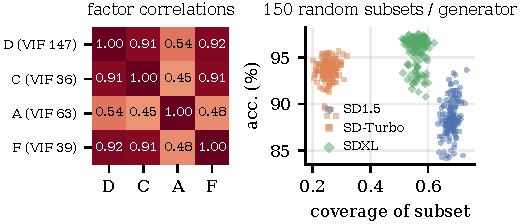
\includegraphics[width=\columnwidth]{figs/fig3.pdf}
\caption{\textbf{Why attribution fails at pilot scale.} \textbf{Left:} correlations and variance-inflation factors of the four factors across 450 random subsets; $D$, $C$ and $F$ are nearly collinear. \textbf{Right:} subsets vary mostly \emph{between} pools; within a pool, coverage moves little.}\label{fig:collin}
\end{figure}

\subsection{Where the gap lives (H3)}\label{sec:h3}
\begin{figure}[t]
\centering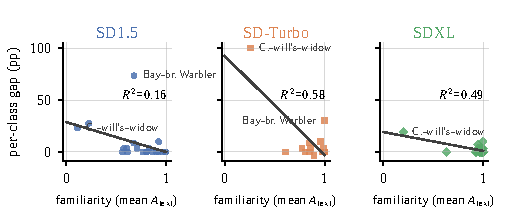
\includegraphics[width=\columnwidth]{figs/fig4.pdf}
\caption{\textbf{Where the gap lives.} Per-class accuracy gap (real minus synthetic, P1) against class familiarity, with OLS fits. Most classes have no gap; two account for 58--82\% of it. SD-Turbo's Bay-breasted Warbler has a 30-point gap at familiarity 0.995.}\label{fig:gap}
\end{figure}
\paragraph{A few classes carry the gap.} 55--65\% of classes show no gap at all, and the two worst classes account for 65\%, 82\% and 58\% of the summed per-class gap for SD1.5, SD-Turbo and SDXL (Fig.~\ref{fig:gap}). The least familiar class is the same for all three generators, Chuck-will's-widow (familiarity 0.11--0.25); trained on SD-Turbo images, the probe gets none of its test images right.

\paragraph{H3 is only weakly supported, and familiarity can be confidently wrong.} The gap falls with familiarity for all three generators (slopes $-0.29$, $-0.95$, $-0.18$), with OLS $R^2$ of 0.16, 0.58 and 0.49 ($p{=}0.085$, $10^{-4}$, $6\cdot10^{-4}$). But because gaps are zero-inflated, the 95\% bootstrap intervals contradict OLS: they exclude zero only for SD1.5. The outliers are instructive. SD1.5's Bay-breasted Warbler has a 73-point gap at moderate familiarity (0.68), and for SD-Turbo the same species has a 30-point gap although CLIP assigns its images a mean zero-shot probability of 0.995. A text scorer can be certain that an image shows the prompted species while the image lacks the cues that distinguish it, so $\Atext$ under-detects exactly the failures that matter.

\subsection{DAS against its ablations (H4)}\label{sec:das-res}
\paragraph{DAS helps consistently, mostly through its filter.} DAS-real improves on Random-$N$ by $+2.4$, $+2.1$ and $+1.2$ points and DAS-text by $+3.4$, $+1.2$ and $+1.2$ (Tab.~\ref{tab:das}, Fig.~\ref{fig:das}), closing 25--44\% of the gap to Real-$N$. Only one gain is individually significant under our conservative test (DAS-text on SD1.5, $p{=}0.03$), but all six are positive (two-sided sign test $p{=}0.03$). DAS beats training on the whole $3\times$ pool in 5/6 settings, so its gain is not simply more images. However, a plain alignment filter equals or beats DAS in three of six settings, and $k$-center alone \emph{hurts} for SD1.5 and SD-Turbo ($-2.1$, $-1.4$), as expected if farthest-point selection seeks out misaligned outliers. The ordering inside DAS, filter first and only then spread, is what makes the coverage step harmless; we cannot credit it with a gain of its own. Like the factorial, DAS helps the weakest generator most, again pointing to alignment as the fixable deficit.

\begin{table}[t]
\centering\scriptsize
\setlength{\tabcolsep}{1.5pt}
\begin{tabular}{@{}lcrrrrrr@{}}
\toprule
 & Real & \multicolumn{2}{c}{SD1.5} & \multicolumn{2}{c}{SD-Turbo} & \multicolumn{2}{c}{SDXL} \\
Method & /cls & Acc & $\Delta$ & Acc & $\Delta$ & Acc & $\Delta$ \\
\midrule
Random-N & 0 & 90.6 & 0 & 93.8 & 0 & 95.9 & 0 \\
All-$mN$ (3$\times$ images) & 0 & 90.4 & $-$0.02 & 95.4 & +0.32 & 96.2 & +0.12 \\
$k$-center only & 0 & 88.5 & $-$0.26 & 92.5 & $-$0.29 & 96.6 & +0.25 \\
Filter only ($A_\text{text}$) & 0 & 91.6 & +0.13 & \textbf{96.2} & +0.50 & \textbf{97.3} & +0.50 \\
DAS-text & 0 & \textbf{94.0}$^*$ & +0.43 & 95.0 & +0.25 & 97.1 & +0.44 \\
\midrule
Filter only ($A_\text{real}$) & 5 & 90.6 & +0.00 & 95.2 & +0.29 & \textbf{97.3} & +0.50 \\
DAS-real & 5 & 93.0 & +0.30 & 95.9 & +0.43 & 97.1 & +0.44 \\
\midrule
Real 5-shot + DAS-real & 5 & 97.9 & +0.91 & 98.5 & +0.96 & 97.6 & +0.62 \\
Real 5-shot (no synthetic) & 5 & \multicolumn{6}{c}{97.8} \\
Real-$N$ (reference) & all & \multicolumn{6}{c}{98.6} \\
\midrule
\multicolumn{8}{@{}l}{\emph{DAS-real ablations (accuracy)}} \\
\quad $\tau$ = 20th pct. & 5 & \multicolumn{2}{c}{93.2} & \multicolumn{2}{c}{95.0} & \multicolumn{2}{c}{96.4} \\
\quad $\tau$ = 40th pct.\ (default) & 5 & \multicolumn{2}{c}{93.0} & \multicolumn{2}{c}{95.9} & \multicolumn{2}{c}{97.1} \\
\quad $\tau$ = 60th pct. & 5 & \multicolumn{2}{c}{93.3} & \multicolumn{2}{c}{96.1} & \multicolumn{2}{c}{97.4} \\
\quad centroid-nearest anchor & 5 & \multicolumn{2}{c}{94.4} & \multicolumn{2}{c}{95.7} & \multicolumn{2}{c}{97.3} \\
\bottomrule
\end{tabular}
\caption{\textbf{DAS versus its ablations} (P2, 480 images unless noted). $\Delta$: fraction of gap closed (Eq.~\ref{eq:delta}). Bold: best synthetic-only set. $^*$: $p{<}0.05$ vs.\ Random-$N$ under a conservative unpaired test; one test image is 0.17 points. Real 5-shot was re-trained in this stage and differs from Tab.~\ref{tab:main} by one test image.}
\label{tab:das}
\end{table}


\begin{figure}[t]
\centering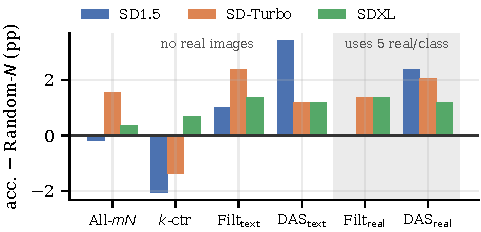
\includegraphics[width=\columnwidth]{figs/fig5.pdf}
\caption{\textbf{Gain over Random-$N$} (480 images, P2). $k$-center alone hurts weaker generators; filtering by alignment carries most of DAS's benefit.}\label{fig:das}
\end{figure}

\paragraph{Real images still win.} Five real images per class (97.8\%) beat every synthetic-only set, including the best one (97.3\%); adding DAS-real images to them changes accuracy by $-0.2$ to $+0.7$ points. Likewise, adding 480 synthetic images (random or DAS) to 5 or 10 real images per class moves accuracy by $-0.5$ to $+0.9$ points. With real-only accuracy near 98\% on these 20 classes, the pilot cannot locate the real-data budget beyond which synthetic data stops helping.

\paragraph{Ablations.} Moving $\tau$ between the 20th and 60th percentile changes DAS-real by about one point at most (1.0 for SD-Turbo and SDXL, 0.3 for SD1.5). Seeding $k$-center at the point nearest the class centroid instead of the most aligned image gives $+1.4$ for SD1.5 and $\le$0.2 otherwise, so our default anchor is not optimal and should be revisited at full scale.

\paragraph{Qualitative failure modes.} Figure~\ref{fig:fail} shows what alignment filtering discards. In our reading, low-scoring images fall into three groups: the bird is tiny or occluded in a scene that the diversified prompt emphasized, the anatomy is wrong (fused puffin--duck shapes), or the image shows a different species. The top row is a reminder that $\Areal$ errs too: several plausible Savannah Sparrows score low, so filtering also discards some correct images.

\begin{figure}[t]
\centering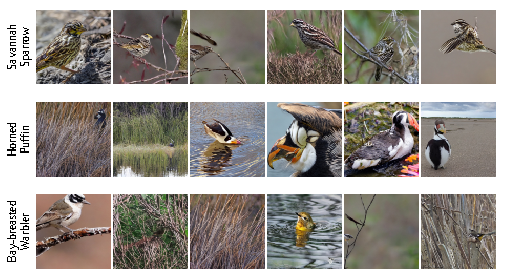
\includegraphics[width=\columnwidth]{figs/fig6.pdf}
\caption{\textbf{What the filter removes.} The six lowest-$\Areal$ SD1.5 (P2) images for three classes chosen by a fixed random rule (rows are not hand-picked). Failures include a bird too small to identify (most rows), anatomically wrong puffins, and a different species (bottom left). The top row also shows the cost of a 5-shot scorer: several plausible sparrows score low.}\label{fig:fail}
\end{figure}

%-------------------------------------------------------------------------
\section{Discussion and limitations}\label{sec:limits}
\paragraph{What the interventions identify.} Selecting from a fixed pool removes the confounds that cross-generator comparisons cannot: architecture, autoencoder, training data and sampler. It does not make the four factors exhaustive. An unmeasured property that co-varies with a selection rule, such as texture statistics~\cite{adamkiewicz2026pretty} or background clutter, is absorbed into the factor it travels with; the manipulation checks in Tab.~\ref{tab:factorial} show that arms move several factors at once. The decomposition says which \emph{measured} property, when manipulated, moves accuracy, not why a pool looks the way it does.

\paragraph{What was not run.} (i) 20 of 200 CUB classes; they are easy (real data reaches 98.6\%), which compresses differences. (ii) Three generators, one generation seed per pool and 585 test images; many DAS differences are one to six images. (iii) SD3.5 and FLUX.1-dev, the models the title question is really about, plus FGVC-Aircraft, the P3 caption regime, SDXL's autoencoder ceiling, a from-scratch ResNet control, CLIP-space and $\Atext$ re-runs of the decomposition, and the $m$ and selection-embedding ablations. (iv) 150 instead of 500 random subsets, without intervals on Shapley shares. (v) SD-Turbo's unusually low P1 precision and coverage (0.03 each) should be checked before being relied on. (vi) A third mixing condition (all real images plus synthetic) is omitted: an implementation error trained it without the real images, and it was not re-run.

\paragraph{Scope of the learner.} The probe measures synthetic images as supervision for a head on a strong real-pretrained backbone, not as pretraining data. Generators and DINOv2 may have seen CUB images; this would inflate synthetic and probe accuracy alike and bias toward synthetic data. DAS-real needs five real images per class; DAS-text needs none but inherits CLIP's blind spots on fine-grained classes (Sec.~\ref{sec:h3}).

\paragraph{Implications.} Within this scope: (i) for a weak generator, check label alignment before chasing diversity; a free CLIP zero-shot filter gave the largest single gain. (ii) Do not rank generators as data sources by precision; here $\FDD$ tracked utility and precision inverted it. (iii) Diversity metrics computed without a reference reward spread into the wrong places; measure coverage of real data instead. (iv) When a handful of real images exist, use them directly. (v) Generator developers who want their models used as data sources should report per-class label alignment on fine-grained classes, judged by a scorer other than CLIP.

\paragraph{Data, licences and impact.} We use a published dataset under its research terms and open generators under their non-commercial licences, and collect no human-subject data. The foreseeable risk is over-confidence: a recipe that narrows the gap on benchmarks could encourage substituting synthetic for real data in high-stakes domains where generator failures are hardest to see; our results, including where DAS does not help, argue for real-data validation there. Code, configurations and selection indices will be released.

\section*{LLM Usage Statement}
Claude (Anthropic) was used extensively in this work, mostly as an autonomous agent working from the authors' research plan. \emph{Code:} it wrote the experiment and analysis code and ran the analysis stages. \emph{Experiments:} it carried out the statistical analysis of the stored outputs and drafted the interpretation of the results. \emph{Figures and tables:} all were generated by scripts it wrote, directly from stored outputs; no number was edited or selected by hand. \emph{Text and related work:} it drafted and revised every section, including the related-work section, and compiled the bibliography. \emph{Data:} the P2 prompt templates were written with an LLM ([authors: name and version]). The research question, hypotheses and study design come from the authors' plan. The authors reviewed all content and take full responsibility for it.

{\small
\bibliographystyle{ieeenat_fullname}
\bibliography{refs}
}
\end{document}
